\documentclass[12pt]{scrartcl}

% packages
\usepackage[
    a4paper, total={18cm, 26cm},
    left=0.75in,
    right=0.75in,
    top=0.75in,
    bottom=0.50in,
    footskip=15pt
]{geometry}
\usepackage{lastpage}
\usepackage{graphicx} % \includegraphics
\usepackage{amsmath, esint} % math
\usepackage{steinmetz} % \phase
\usepackage{import} % \import
\usepackage{esdiff} % \diff
\usepackage{fancyhdr} % header and footer
\usepackage{listings}

\makeatletter
\def\today{%
  \two@digits{\the\day}/%
  \ifcase\month\or%
  01\or 02\or 03\or 04\or 05\or 06\or%
  07\or 08\or 09\or 10\or 11\or 12\fi/%
  \number\year%
}
\makeatother

% configs
\setlength{\parindent}{0pt}

% comandos
\renewcommand{\familydefault}{\sfdefault}
\newcommand{\un}[1]{\;\textrm{#1}}
\newcommand{\logo}{\quad \Rightarrow \quad}
\newcommand{\fase}[1]{\ensuremath{\phase{{#1}^{\circ}}}}

\newcommand*\VF[1]{\mathbf{#1}}
\newcommand*\dif{\mathop{}\!\mathrm{d}}


\begin{document}

\pagestyle{fancy}

\fancyhead{}
\fancyhead[L]{Python Aplicado a Sinais e Sistemas - PET Engenharias}
\fancyhead[R]{Data: \today}
\fancyfoot{}
\fancyfoot[R]{Pág. \thepage \; / \pageref{LastPage}}

\begin{center}
    Aluno: Raphael Henrique Braga Leivas \\[20pt]
    Email: rapha.lei8@gmail.com
\end{center}

\hrule

\section*{Atividade 6 - Capítulo 7}

O código completo usado nessa atividade se encontra no ANEXO A.

\subsection*{Exercício 2}

\begin{figure}[htp!]
	\begin{center}
    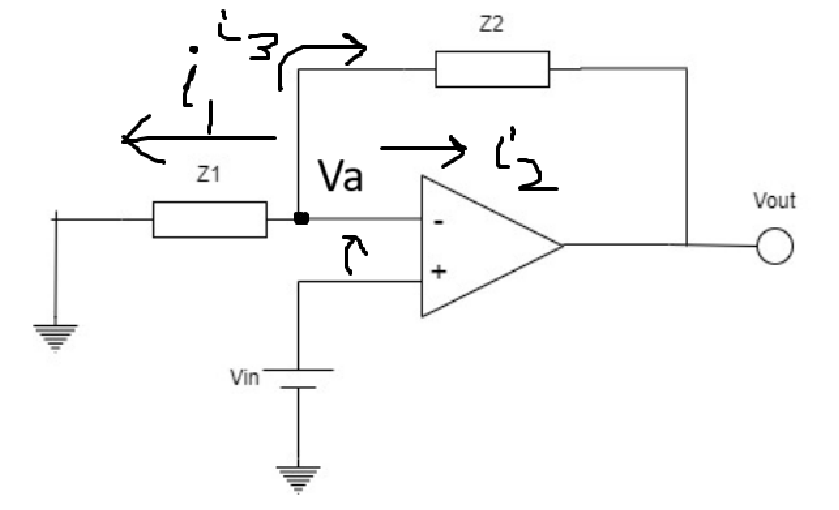
\includegraphics[width=0.8\textwidth,trim=1 1 1 1,clip]{ex2.png}
	\end{center}
\end{figure}

Aplicando análise nodal em $V_a$, temos

\[ i_1 + i_2 + i_3 = 0  \]

Note que $i_2 = 0$ pois o AmpOp é ideal e possui impedância de entrada infinita.

\[ \frac{V_a - 0}{Z_1} + 0 + \frac{V_a - V_{out}}{Z_2} = 0  \]

Pelo curto circuito virtual entre as entradas inversora e não-inversora, temos $V_a = V_{in}$. Logo,

\[ \frac{V_{in} - 0}{Z_1} + 0 + \frac{V_{in} - V_{out}}{Z_2} = 0  \]

\[ V_{in} \left(\frac{1}{Z_1} + \frac{1}{Z_2}\right) = V_{out} \frac{1}{Z_2}  \]

\[ \frac{V_{in}}{V_{out}} = G = H(s) = \frac{Z_2}{Z_1} + 1  \]

Suponha que em $Z_2$ temos um capacitor de capacitância $C = 100 nF$ e em $Z_1$
um resistor $R = 1 k\Omega$. Temos

\[ H(s) = \frac{\frac{1}{Cs}}{R} + 1 = \frac{1}{RCs} + 1 \]

A resposta em frequência do circuito é dada pelo Diagrama de Bode abaixo.
Ele atenua frequências maiores que 1 kHz.

\begin{figure}[h!]
	\begin{center}
    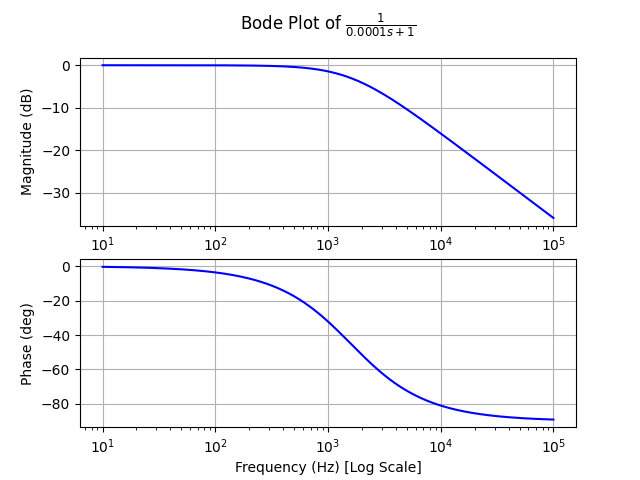
\includegraphics[width=0.8\textwidth,trim=1 1 1 1,clip]{ex2_bode.png}
	\end{center}
\end{figure}


Assumindo que a entrada é uma senoide dada por

\[ x(t) = A \sin (\omega t) \Longrightarrow X(s) = \frac{A \omega}{\omega^{2} + s^{2}} \]

Logo, a saída do sistema é  

\[ Y(s) = X(s) H(s) =  \frac{A \omega}{\left(\omega^{2} + s^{2}\right) \left(C R s + 1\right)} \]

Assumindo $\omega = 1 rad / s$ e $A = 10$, temos a saída com forma de onda abaixo.
O sinal possui a mesma amplitude da entrada.

\begin{figure}[htp!]
	\begin{center}
    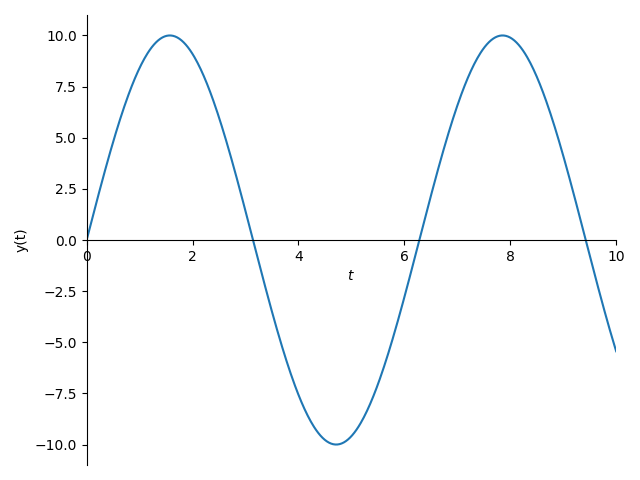
\includegraphics[width=0.8\textwidth,trim=1 1 1 1,clip]{ex2_baixaf.png}
	\end{center}
\end{figure}

Se a entrada tivesse frequência maior, $\omega = 10 krad / s$,
temos a forma de onda abaixo. O sinal é atenuado em alta frequência, 
deformando-se e possuindo amplitude menos que a entrada.

\begin{figure}[htp!]
	\begin{center}
    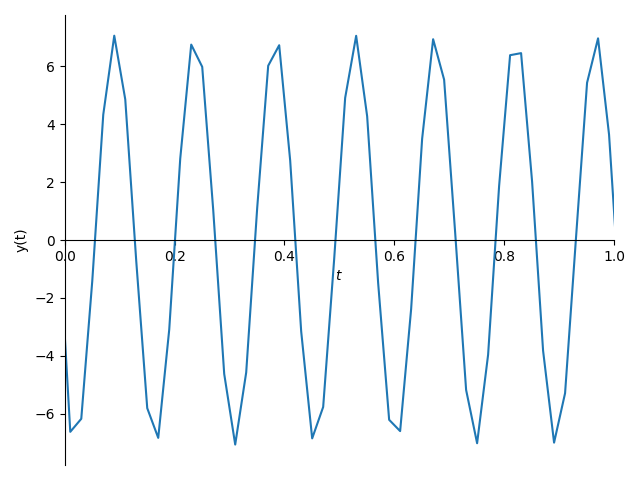
\includegraphics[width=0.8\textwidth,trim=1 1 1 1,clip]{ex2_altaf.png}
	\end{center}
\end{figure}

\newpage

\section*{ANEXO A - Código}

\begin{lstlisting}[language=Python, breaklines=true, basicstyle=\scriptsize]
    import numpy as np
    import matplotlib as plt
    from sympy import *
    from sympy.physics.control.control_plots import pole_zero_plot
    from sympy.physics.control.control_plots import bode_plot
    from sympy.physics.control.lti import TransferFunction
    
    ## Exercicio 2
    
    t, s = symbols('t, s')
    omega, A = symbols('omega, A')
    xt = A * sin(omega*t)
    
    Xs = laplace_transform(xt, t, s, noconds=True)
    
    print(latex(Xs))
    
    C, R = symbols('C, R')
    
    Hs_num = 1
    Hs_den = R * C * s + 1
    
    ft1 = TransferFunction(Hs_num, Hs_den, s)
    
    # bode_plot(ft1.subs({ C: 100e-9, R: 1e3 }), initial_exp=1, final_exp=5, phase_unit='deg', freq_unit='Hz')
    
    Ys = Xs * (Hs_num / Hs_den)
    
    yt = inverse_laplace_transform(Ys.subs({ C: 100e-9, R: 1e3, A: 10, omega: 10000 }), s, t, noconds=True)
    
    print(latex(yt))
    
    plot(yt, ylabel = "y(t)", xlim=(0, 1))    
\end{lstlisting}

\end{document}